
%<<setup-child, include = FALSE>>=
%library(knitr)
%library(ggplot2)
%set_parent("../style/preamble.Rnw")
%options(digits = 16)
%@

\input{../../2021/style/preamble4tex}
% dependencies: amsmath, amssymb, dsfont
% math spaces
\ifdefined\N
\renewcommand{\N}{\mathds{N}} % N, naturals
\else \newcommand{\N}{\mathds{N}} \fi
\newcommand{\Z}{\mathds{Z}} % Z, integers
\newcommand{\Q}{\mathds{Q}} % Q, rationals
\newcommand{\R}{\mathds{R}} % R, reals
\ifdefined\C
\renewcommand{\C}{\mathds{C}} % C, complex
\else \newcommand{\C}{\mathds{C}} \fi
\newcommand{\continuous}{\mathcal{C}} % C, space of continuous functions
\newcommand{\M}{\mathcal{M}} % machine numbers
\newcommand{\epsm}{\epsilon_m} % maximum error

% counting / finite sets
\newcommand{\setzo}{\{0, 1\}} % set 0, 1
\newcommand{\setmp}{\{-1, +1\}} % set -1, 1
\newcommand{\unitint}{[0, 1]} % unit interval

% basic math stuff
\newcommand{\xt}{\tilde x} % x tilde
\newcommand{\argmin}{\mathop{\mathrm{arg\,min}}} % argmin
\newcommand{\argmax}{\mathop{\mathrm{arg\,max}}} % argmax
\newcommand{\argminlim}{\argmin\limits} % argmin with limits
\newcommand{\argmaxlim}{\argmax\limits} % argmax with limits
\newcommand{\sign}{\operatorname{sign}} % sign, signum
\newcommand{\I}{\mathbb{I}} % I, indicator
\newcommand{\order}{\mathcal{O}} % O, order
\newcommand{\bigO}{\mathcal{O}} % Big-O Landau
\newcommand{\littleo}{{o}} % Little-o Landau
\newcommand{\pd}[2]{\frac{\partial{#1}}{\partial #2}} % partial derivative
\newcommand{\floorlr}[1]{\left\lfloor #1 \right\rfloor} % floor
\newcommand{\ceillr}[1]{\left\lceil #1 \right\rceil} % ceiling
\newcommand{\indep}{\perp \!\!\! \perp} % independence symbol

% sums and products
\newcommand{\sumin}{\sum\limits_{i=1}^n} % summation from i=1 to n
\newcommand{\sumim}{\sum\limits_{i=1}^m} % summation from i=1 to m
\newcommand{\sumjn}{\sum\limits_{j=1}^n} % summation from j=1 to p
\newcommand{\sumjp}{\sum\limits_{j=1}^p} % summation from j=1 to p
\newcommand{\sumik}{\sum\limits_{i=1}^k} % summation from i=1 to k
\newcommand{\sumkg}{\sum\limits_{k=1}^g} % summation from k=1 to g
\newcommand{\sumjg}{\sum\limits_{j=1}^g} % summation from j=1 to g
\newcommand{\summM}{\sum\limits_{m=1}^M} % summation from m=1 to M
\newcommand{\meanin}{\frac{1}{n} \sum\limits_{i=1}^n} % mean from i=1 to n
\newcommand{\meanim}{\frac{1}{m} \sum\limits_{i=1}^m} % mean from i=1 to n
\newcommand{\meankg}{\frac{1}{g} \sum\limits_{k=1}^g} % mean from k=1 to g
\newcommand{\meanmM}{\frac{1}{M} \sum\limits_{m=1}^M} % mean from m=1 to M
\newcommand{\prodin}{\prod\limits_{i=1}^n} % product from i=1 to n
\newcommand{\prodkg}{\prod\limits_{k=1}^g} % product from k=1 to g
\newcommand{\prodjp}{\prod\limits_{j=1}^p} % product from j=1 to p

% linear algebra
\newcommand{\one}{\bm{1}} % 1, unitvector
\newcommand{\zero}{\mathbf{0}} % 0-vector
\newcommand{\id}{\bm{I}} % I, identity
\newcommand{\diag}{\operatorname{diag}} % diag, diagonal
\newcommand{\trace}{\operatorname{tr}} % tr, trace
\newcommand{\spn}{\operatorname{span}} % span
\newcommand{\scp}[2]{\left\langle #1, #2 \right\rangle} % <.,.>, scalarproduct
\newcommand{\mat}[1]{\begin{pmatrix} #1 \end{pmatrix}} % short pmatrix command
\newcommand{\Amat}{\mathbf{A}} % matrix A
\newcommand{\Deltab}{\mathbf{\Delta}} % error term for vectors

% basic probability + stats
\renewcommand{\P}{\mathds{P}} % P, probability
\newcommand{\E}{\mathds{E}} % E, expectation
\newcommand{\var}{\mathsf{Var}} % Var, variance
\newcommand{\cov}{\mathsf{Cov}} % Cov, covariance
\newcommand{\corr}{\mathsf{Corr}} % Corr, correlation
\newcommand{\normal}{\mathcal{N}} % N of the normal distribution
\newcommand{\iid}{\overset{i.i.d}{\sim}} % dist with i.i.d superscript
\newcommand{\distas}[1]{\overset{#1}{\sim}} % ... is distributed as ...


\begin{document}

\lecturechapter{5}{Laplace's method}
\lecture{CIM1 Statistical Computing}



%\section{Laplace's method}

\begin{vbframe}{Laplace's method}

%<<out.width = '90%', fig.align = "center", echo = FALSE>>=
%# Berechne Posterior für Gamma
%makepost = function(y, shape, scale) {
%        function(x) {
%          dgamma(x, shape = y + shape, scale = 1 / (1 + 1 / scale))
%        }
%}
%@

\textbf{Target:} Approximate integral of function $f$ with the following properties:

\begin{itemize}
\item The mass concentrates on a small area around a center and the function has very rapidly decreasing tails
%approaches $0$ fast for $x \to \pm \infty$ 
(\enquote{similarity} to the density of a normal distribution)
\item The function we want to integrate is the density of a random variable that is approximately normally distributed
\end{itemize}

% Genauer gesagt fordern wir $f \in \mathcal{L}^2$ (quadratische Integrierbarkeit)
%
% \vspace*{-0.1cm}
%
% $$
% \int f(x)^2 dx < \infty.
% $$


\begin{center}
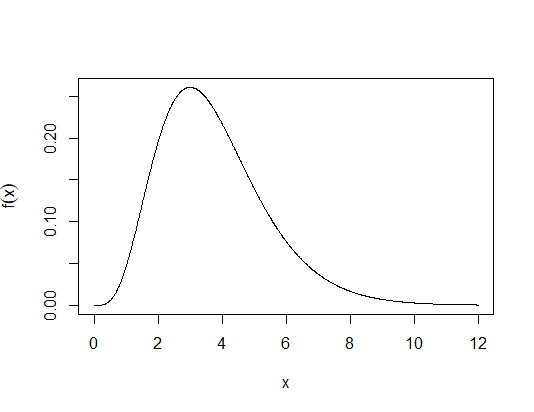
\includegraphics[width =0.5\textwidth]{figure_man/normaldist.png}
\end{center}

%<<out.width = '60%', fig.align = "center", echo = FALSE>>=
%# We're already using the Gamma Posterior distribution here
%# as example function
%# Later we'll explain the example in more detail
%# So far this is just "some" example function
%set.seed(1234)

%y = 2
%prior.shape = 3
%prior.scale = 3

%p = makepost(y, prior.shape, prior.scale)

%pmode = (y + prior.shape - 1) * (1 / (1 + 1 / prior.scale))
%pmean = (y + prior.shape) * (1 / (1 + 1 / prior.scale))

%a = prior.shape
%b = prior.scale

%fhat = deriv3(~ mu^(y + a - 1) * exp(-mu * (1 + 1/b)) / ((1/(1+1/b))^(y+a) * gamma(y + a)), "mu", function.arg = TRUE)

%post.shape = y + prior.shape - 1
%post.scale = 1 / (length(y) + 1 / prior.scale)

%curve(p, 0, 12, n = 1000, xlab = expression(x), ylab = expression(f(x)))
%@



\framebreak
In particular, we assume that $f$

\begin{itemize}
\item Can only be positive
\item Is two times continuously differentiable
\item Has a \textbf{global maximum} at $x_0$
\end{itemize}


%\framebreak
\vspace*{0.1cm}
We could approximate the area underneath the graph of the function with a staircase function and represent the integral with a very simple formula that depends on $f(x_0)$:
\vspace*{-0.1cm}
\begin{footnotesize}
$$
\int f(x)~dx \approx f(x_0) \cdot c
$$

\begin{center}
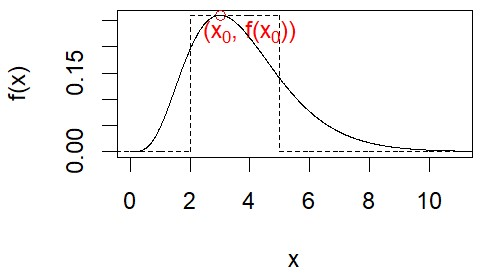
\includegraphics[width =0.5\textwidth]{figure_man/normaldist2.jpg}
\end{center}

%<<out.width = '59%', fig.align = "center", echo = FALSE>>=
%par(cex = 1.5)

%y0 = 0.26 * c(0, 0, rep(1, 3), rep(0, 6))
%sfun = stepfun(1:10, y0, f = 0)
%plot(sfun, main = "", lty = 2, do.points = FALSE)
%points(3, p(3), col = "red")
%text(x = 4, 0.23, expression(paste("(", x[0], ", f(", x[0], "))")), col = "red")
%curve(p, 0, 12, n = 1000, xlab = expression(x), ylab = expression(f(x)), add = TRUE)
%@
\end{footnotesize}

\framebreak

But instead of the step function we would like to choose a function that approximates $f$ \textbf{better} and which has well-known properties.

\lz

\textbf{Idea:} Approximate the integral using the density function of the normal distribution!

\lz

\textbf{How?} We center and scale the density function of the normal distribution such that it approximates $f$ \enquote{best possible}.

\framebreak

In other words: We determine \textbf{expectation} and \textbf{standard deviation} of a normal distribution such that the corresponding density function fits best possible to the function $f$ we are interested in.

\begin{center}
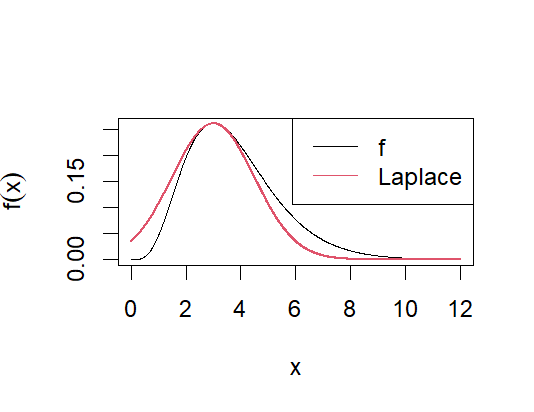
\includegraphics[width =0.7\textwidth]{figure_man/laplace01.png}
\end{center}


\framebreak

\textbf{Mathematical derivation:}

Let there be a function $f$ with a global maximum at $x_0$.

\lz

We define $h(x) := \log f(x)$ as the logarithmized function and rewrite the integral

$$
\int_a^b f(x)~dx = \int_a^b \exp(\underbrace{\log f(x)}_{:=h(x)})~dx
$$

Using Taylor's theorem around $x_0$ we obtain

\small
$$
\int_a^b \exp\left(h(x)\right) \approx \int_a^b \exp\left( h(x_0) + h'(x_0)(x - x_0) + \frac{1}{2} h''(x_0)(x - x_0)^2\right) dx
$$
\normalsize

\framebreak

$x_0$ is also the maximum of $h(x) = \log(f(x))$ . Hence, $h'(x_0) = 0$ and the second summand disappears:

$$
\int_a^b \exp\left(h(x)\right)~dx \approx \int_a^b \exp\left( h(x_0) + \frac{1}{2} h''(x_0)(x - x_0)^2\right) dx
$$

We take advantage of the fact that $\exp(x + y) = \exp(x)\exp(y)$

$$
\int_a^b \exp\left( h(x_0)\right) \cdot \exp\left(\frac{1}{2} h''(x_0)(x - x_0)^2\right) dx
$$

and pull the constant $\exp\left( h(x_0)\right)$ out of the integral

$$
\exp\left( h(x_0)\right) \cdot\int_a^b \exp\left(\frac{1}{2} h''(x_0)(x - x_0)^2\right) dx
$$

\framebreak

Within the integral there is now an expression which \enquote{almost} corresponds to the density of a normal distribution with expectation $\mu := x_0$ and variance $\sigma^2 := -h''(x_0)^{-1}$:

\vspace{-0.3cm}

\begin{eqnarray*}
\int_a^b f(x) dx &\approx& \exp\left( h(x_0)\right) \cdot\int_a^b  \exp\left(\frac{1}{2} h''(x_0)(x - x_0)^2\right)~dx \\
&=& \exp\left( h(x_0)\right) \cdot\int_a^b  \exp\left(-\frac{1}{2} \frac{(x - x_0)^2}{-h''(x_0)^{-1}}\right) ~dx\\
&=& \exp\left( h(x_0)\right) \cdot\int_a^b  \exp\left(-\frac{1}{2} \frac{(x - \mu)^2}{\sigma^2}\right)~dx
\end{eqnarray*}

\vfill

\begin{footnotesize}
$-h''(x_0)^{-1}$ must be truly positive to correspond to the variance of a normal distribution. Since $h(x)$ has a global maximum in $x_0$, the second derivative at this point is negative and therefore $-h''(x_0)^{-1} > 0$.
\end{footnotesize}

\framebreak

If we add (and cancel) the multiplicative constant $c = \frac{1}{\sqrt{2\pi\sigma^2}}$, we obtain

\begin{eqnarray*}
\int_a^b f(x) dx &\approx& \frac{1}{c} \cdot \exp\left( h(x_0)\right) \cdot\int_a^b \underbrace{c \cdot \exp\left(-\frac{1}{2} \frac{(x - \mu)^2}{\sigma^2}\right)}_{\text{Density ND}}~dx\\
&=& \frac{1}{c}\underbrace{\exp\left( h(x_0)\right)}_{f(x_0)} \cdot \int_a^b \phi_{\mu, \sigma^2} (x)~dx \\
&=& \frac{1}{c}f(x_0) \cdot \left(\Phi_{\mu, \sigma^2}(b) - \Phi_{\mu, \sigma^2}(a)\right)
\end{eqnarray*}

where $\phi_{\mu, \sigma^2}(x)$ denotes the density and $\Phi_{\mu, \sigma^2}(x)$ the distribution function of a normal distribution with expectation $\mu$ and variance $\sigma^2$.

\framebreak

For integration limits $b = \infty$ and $a = -\infty$ Laplace's method of $f$ is then

\begin{eqnarray*}
\int_{-\infty}^{\infty} f(x) dx &\approx& \frac{1}{c}\cdot f(x_0) \cdot \left(\Phi_{\mu, \sigma^2}(+ \infty) - \Phi_{\mu, \sigma^2}(-\infty)\right) \\
&=& \sqrt{- \frac{2\pi}{h''(x_0)}} \cdot f(x_0)
\end{eqnarray*}

with $h(x) = \log f(x)$.

\lz

Laplace's method thus corresponds to a value that only depends on the maximum of the function $f(x_0)$ and the curvature of the logarithmic function $h''(x_0)$.
\framebreak

Laplace's method also works well in higher dimensions. For $f:\R^{m} \to \R$ with global maximum in $\bm{x}_0$ the generalized form is given by

\begin{eqnarray*}
I(f) &\approx& (2\pi)^{m/2} \det(-H_f(x_0)^{-1})^{1/2} \exp(f(x_0))
\end{eqnarray*}

where $H_f(x_0)$ denotes the Hessian matrix of $f$ at $x_0$. Since $x_0$ is a global maximum, $H_f(x_0)$ is negative definite.

%\framebreak
\lz

The problem of integration is reduced to

\begin{itemize}
\item Solving an optimization problem $\to$ find $x_0$
\item Determining the second derivative $h''(x)$ (or generally the Hessian matrix $H_f(\bm{x})$) at the optimal position $x_0$.
\end{itemize}

Instead of integration, an optimization problem must now be solved, which is often much easier and faster.

% \item Analytische Ergebnisse können verwendet werden, um den numerischen Fehler abzuschätzen.


\end{vbframe}

\begin{vbframe}{Laplace's method: example}

\textbf{Application example:} Bayesian computation

\lz

\textbf{Given}:

\vspace*{-0.8cm}
\begin{eqnarray*}
x | \lambda &\sim& \text{Poisson}(\lambda) \quad \text{(Likelihood)}\\
\lambda &\sim& \text{Gamma}(\alpha, \beta) \quad \text{(Prior)}
\end{eqnarray*}

\textbf{Wanted}: Posterior density of the parameter $\lambda$ given $n$ observations $\bm{x} = \left(x^{(1)}, x^{(2)}, ..., x^{(n)}\right)$

$$
\overset{Posterior}{p(\lambda | \bm{x})} = \frac{\overset{Likelihood}{p(\bm{x} | \lambda)} \cdot \overset{Prior}{\pi(\lambda)}}{\int p(\bm{x} | \lambda) \cdot \pi(\lambda) ~ d\lambda}
$$

\vfill

\begin{footnotesize}
The density of the gamma distribution is given by $\pi_{\alpha, \beta}(\lambda) = \frac{1}{\beta^\alpha\Gamma(\alpha)}\lambda^{\alpha-1}\exp(-\lambda \beta)$
\end{footnotesize}

\framebreak

To keep the calculations simple, we calculate the posterior density for only \textbf{one} observation $x$.

\lz

The posterior density of $\lambda$ given the observation $x$ is (except for one constant)

$$
p(\lambda | x) \propto \lambda^{x + \alpha - 1} \exp\left(- \frac{\lambda}{1 / \beta + 1}\right) =: f(\lambda).
$$

So to determine the posterior density $p(\lambda|x)$ \textbf{exactly}, we search for the normalization constant $c$, which ensures that $\int c \cdot f(\lambda) ~d\lambda = 1$, hence
\vspace*{-0.3cm}
\begin{eqnarray*}
c \cdot \int f(\lambda) ~ d\lambda &=& 1 \\
c  &=& \frac{1}{\int f(\lambda)~d\lambda}
\end{eqnarray*}

\framebreak

\textbf{Goal:} Approximation of $\int f(\lambda)~d\lambda$ with $f(\lambda) = \lambda^{x + \alpha - 1} \exp\left(- \frac{\lambda}{1 / \beta + 1}\right)$

\lz

We calculate $h(\lambda) = \log f(\lambda)$

\vspace*{-0.5cm}
\begin{eqnarray*}
h(\lambda) &=& \log \left(\lambda^{x + \alpha - 1}\cdot\exp(-\frac{\lambda}{1 / \beta + 1}) \right) \\
&=& \left({x} + \alpha - 1\right) \log \lambda - \frac{\lambda}{1 / \beta + 1} \\
h'(\lambda) &=& \frac{x + \alpha - 1}{\lambda} - \frac{1}{1 / \beta + 1} \\
h''(\lambda) &=& - \frac{x + \alpha - 1}{\lambda^2}
\end{eqnarray*}

\framebreak

To approximate the integral using Laplace's method, we need $\lambda_0 := \text{arg max } f(\lambda)$ and $h''(\lambda_0)$, where $h(\lambda) := \log (f(\lambda))$.

\lz

The maximum of $f(\lambda)$ is the same as the maximum of $h(\lambda)$ (easier to calculate)

\vspace*{-0.5cm}
\begin{eqnarray*}
h'(\lambda) &=& 0\\
\frac{x + \alpha - 1}{\lambda} - \frac{1}{1 / \beta + 1} &=& 0 \\
\lambda_0 &=& \frac{x + \alpha - 1}{1 / \beta + 1}
\end{eqnarray*}

and thus

\vspace*{-0.3cm}

\begin{eqnarray*}
h''(\lambda_0) &=& - \frac{(1 / \beta + 1)^2}{x + \alpha - 1}
\end{eqnarray*}

\framebreak

We insert $\lambda_0 = \frac{x + \alpha - 1}{1 / \beta + 1}$ and $h''(\lambda_0)$ into the formula for Laplace's method and obtain

\begin{eqnarray*}
\int f(\lambda) d\lambda &\approx& \sqrt{- \frac{2\pi}{h''(\lambda_0)}} \cdot f(\lambda_0) \\
&=& \sqrt{2 \pi} \cdot \frac{\sqrt{x + \alpha - 1}}{1 / \beta + 1}\cdot f(\lambda_0)
\end{eqnarray*}

Hence, the normalization constant $c$ can be approximated by

$$
c =\frac{1}{\int f(\lambda) d\lambda} \approx \frac{1}{\sqrt {2\pi}}\frac{1 / \beta + 1}{\sqrt{x + \alpha - 1}}\cdot \frac{1}{f(\lambda_0)}
$$


%<<out.width = '80%', fig.align = "center", echo = FALSE, include = FALSE>>=
%par(cex = 1.5)
%curve(p, 0, 12, n = 1000, lwd = 3, xlab = expression(mu),
%      ylab = expression(paste("p(", mu, " | y)")))
%curve(dgamma(x, shape = prior.shape, scale = prior.scale), add = TRUE,
%      lty = 2)
%legend("topright", legend = c("Posterior", "Prior"), lty = c(1, 2), lwd = c(3, 1), bty = "n")
%@



%<<out.width = '80%', fig.align = "center", echo = FALSE, include = FALSE>>=
%lapprox = Vectorize(function(mu, mu0 = pmode) {
%        deriv = fhat(mu0)
%        grad = attr(deriv, "gradient")
%        hess = drop(attr(deriv, "hessian"))
%        f = function(x) dgamma(x, shape = post.shape, scale = post.scale)
%        hpp = (hess * f(mu0) - grad^2) / f(mu0)^2
%        exp(log(f(mu0)) + 0.5 * hpp * (mu - mu0)^2)
%}, "mu")

%curve(p, 0, 12, n = 1000, lwd = 3, xlab = expression(mu),
%      ylab = expression(paste("p(", mu, " | y)")))
%curve(dgamma(x, shape = prior.shape, scale = prior.scale), add = TRUE,
%      lty = 2)
%legend("topright",
%       legend = c("Posterior Density", "Prior Density", "Laplace Approx"),
%       lty = c(1, 2, 1), lwd = c(3, 1, 1), col = c(1, 1, 2), bty = "n")
%curve(lapprox, 0.001, 12, n = 1000, add = TRUE, col = 2, lwd = 2)
%@


\framebreak

When calculating posterior distributions, Laplace's method provides a good approximation if

\begin{itemize}
\item The number $n$ of observations is large
\item The posterior distributions are roughly symmetric
\end{itemize}

\end{vbframe}


% \section{Erwartungswerte bei Bayes}
%
% \begin{vbframe}{Bayesian Computations}
% Gemeinsame posteriorverteilung von $\theta | x$
% $$
% f(\theta | x) = \frac{f(x | \theta)f(\theta)}{f(x)},
% $$
% und
% $$
% f(x) = \int f(x, \theta)d\theta =
%   \int f(x | \theta)f(\theta)d\theta.
% $$
%
% \lz
%
% Posterior-Mittelwert
% $$
% E(\theta | x) = \int \theta f(\theta | x)d\theta.
% $$
%
% \framebreak

% <<>>=
%  x = rnorm(100, mean = 5)
% @
%
% <<>>=
%  logLik = function(theta) {
%   sum(dnorm(x, mean = theta, log = TRUE))
%   }
%
%   logPrior = function(theta) {
%     dgamma(theta, 2, 2, log = TRUE)
%   }
%
%   k1 = function(theta) {
%     logLik(theta) + logPrior(theta)
%   }
%
%  k2 = function(theta) {
%     log(theta) + logLik(theta) + logPrior(theta)
%   }
% @
%
% <<>>=
%  thetah.1 = optimize(k1, maximum = TRUE, lower = 0.00001, upper = 10)
%  thetah.2 = optimize(k1, maximum = TRUE, lower = 0.00001, upper = 10)
%
% @
%
%
%
%
% <<>>=
%  opt = optimize(logPost, maximum = TRUE,
%    lower = 0.00001, upper = 10)
%  opt
% @
%
% <<>>=
%  mode = opt$maximum
%  mode
%  ordinate = opt$objective
% @
%
% <<>>=
%  posterior = Vectorize(function(theta) {
%    exp(logPost(theta) - ordinate)
%  })
% @
%
% <<>>=
%  const = integrate(posterior, lower = -10, upper = 10)$value
%  const
% @
%
% <<>>=
%  norm.posterior = function(theta) {
%    posterior(theta) / const
%  }
% @
%
% <<>>=
% post.mean = integrate(function(theta) theta*norm.posterior(theta),
%   lower = -10, upper = 10)
% post.mean
% @
% % \end{vbframe}





% \begin{vbframe}{Beispiel Laplace Approximation}
% <<>>=
% x = rnorm(100, mean = 5, sd = 1.5)
% @

% <<>>=
% logLik = function(theta) {
%   sum(dnorm(x, mean = theta[1], sd = theta[2], log = TRUE))
% }
% logPrior = function(theta) {
%   dnorm(theta[1], 0, 10, log = TRUE) + dunif(theta[2], 0, 10)
% }
% logPost = function(theta) {
%   logLik(theta) + logPrior(theta)
% }
% @

% <<>>=
% postExp(theta = c(1, 1), logPost)
% postExp(theta = c(1, 1), logPost,
%   g = function(x) { x^2 })
% @
% \end{vbframe}

\endlecture

\end{document}